\chapter{Introduction}
Artificial intelligence is playing more prominent role in our daily lives by demonstrating human intelligence by machines, especially computer systems. The field includes learning, reasoning and self-correction. These can be described as the acquisition of information and rules for using the information, using the rules to reach approximate or definite conclusions. It has become more important to make machines able to communicate through natural language with human or among machines themselves. Learning algorithms for natural language understanding in language translation, reading comprehension have progressed at a rate in recent years that never done before, but that lack ultimate aspects of how humans understand and produce natural language. Mainly humans develop language understanding and producing by being embodied in an environment which they can realize and interact with other humans~\cite{DBLP:journals/corr/abs-1807-03367}.

In many tasks understanding compositional language in context is very complex. Reasoning about sets of objects, quantities, comparisons and spatial relations are required in visual question answering and robot instruction systems. Robust language understanding is required when instructing assembly-line or home assistance robots to manipulate objects in random environments. And this is only partially addressed by existing datasets~\cite{Suhr2017ACO}.

DONE

The problem of interpreting instructions written in natural language has been widely studied since the early days of artificial intelligence.  Mapping instructions to a sequence of executable actions would enable the automation of tasks that currently require human participation~\cite{RL}.

By ``Natural Language" we mean a language that is used for everyday communication by humans; languages like English, Bengali or Portuguese. In contrast to artificial languages such as programming languages and mathematical notations, natural languages have evolved as they pass from generation to generation, and are hard to pin down with explicit rules. Technologies based on NLP are becoming increasingly widespread. For example, phones and handheld computers support predictive text and handwriting recognition; web search engines give access to information locked up in unstructured text; machine translation allows us to retrieve texts written in Chinese and read them in Spanish; text analysis enables us to detect sentiment in tweets and blogs. By providing more natural human-machine interfaces, and more sophisticated access to stored information, language processing has come to play a central role in the multilingual information society~\cite{NLPbook}.

It is easy to get our hands on millions of words of text. What can we do with it, assuming we can write some simple programs? We're all very familiar with text, since we read and write it every day. Here we will treat text as raw data for the programs we write, programs that manipulate and analyze it in a variety of interesting ways.
\section{Robot Navigation}
Navigation refers to the method of determining aspects such as position, speed, and direction during travel. In the pre-modern era, direction and position were determined using an altazimuth, a compass, and a map; these are now considered primitive forms of navigation. As a result of modern developments in science and technology, exact positions and speeds are determined using equipment such as artificial satellites, global navigation satellite system (GNSS), inertial navigation systems (INS), etc~\cite{NAV}.

\section{Automatic Natural Language Understanding}
At a purely practical level, we all need help to navigate the universe of information locked up in text on the Web. Search engines have been crucial to the growth and popularity of the Web, but have some shortcomings. It takes skill, knowledge, and some luck, to extract answers to such questions as: \emph{What tourist sites can I visit between Philadelphia and Pittsburgh on a limited budget? What do experts say about digital SLR cameras? What predictions about the steel market were made by credible commentators in the past week?}  Getting a computer to answer them automatically involves a range of language processing tasks, including information extraction, inference, and summarization, and would need to be carried out on a scale and with a level of robustness that is still beyond our current capabilities.

On a more philosophical level, a long-standing challenge within artificial intelligence has been to build intelligent machines, and a major part of intelligent behaviour is understanding language. For many years this goal has been seen as too difficult. However, as NLP technologies become more mature, and robust methods for analyzing unrestricted text become more widespread, the prospect of natural language understanding has re-emerged as a plausible goal~\cite{NLPbook}.

In this section we describe some language understanding technologies, to give a sense of the interesting challenges that are related to NLP.
\subsection{Word Sense Disambiguation:}
In word sense disambiguation we want to work out which sense of a word was intended in a given context. Consider the ambiguous words serve and dish:

\begin{enumerate}[a.]
    \item serve: help with food or drink; hold an office; put ball into play
    \item dish: plate; course of a meal; communications device    
\end{enumerate}

In a sentence containing the phrase: he served the dish, we can detect that both serve and dish are being used with their food meanings. It's unlikely that the topic of discussion shifted from sports to crockery in the space of three words. This would force us to invent bizarre images, like a tennis pro taking out his or her frustrations on a china tea-set laid out beside the court. In other words, we automatically disambiguate words using context, exploiting the simple fact that nearby words have closely related meanings. As another example of this contextual effect, consider the word by, which has several meanings, e.g.: the book by Chesterton (agentive -- Chesterton was the author of the book); the cup by the stove (locative -- the stove is where the cup is); and submit by Friday (temporal -- Friday is the time of the submitting). Observe in (c) that the meaning of the italicized word helps us interpret the meaning of by.
\begin{enumerate}[a.]
    \item The lost children were found by the searchers (agentive)
    \item The lost children were found by the mountain (locative)
    \item The lost children were found by the afternoon (temporal)    
\end{enumerate}
\subsection{Pronoun Resolution}
A deeper kind of language understanding is to work out "who did what to whom" — i.e., to detect the subjects and objects of verbs. You learnt to do this in elementary school, but it's harder than you might think. In the sentence the thieves stole the paintings it is easy to tell who performed the stealing action. Consider three possible following sentences in (c), and try to determine what was sold, caught, and found (one case is ambiguous).
\begin{enumerate}[a.]
    \item The thieves stole the paintings. They were subsequently sold.
    \item The thieves stole the paintings. They were subsequently caught.
    \item The thieves stole the paintings. They were subsequently found.
\end{enumerate}
Answering this question involves finding the antecedent of the pronoun they, either thieves or paintings. Computational techniques for tackling this problem include anaphora resolution -- identifying what a pronoun or noun phrase refers to -- and semantic role labeling -- identifying how a noun phrase relates to the verb (as agent, patient, instrument, and so on).

\subsection{Generating Language Output}
If we can automatically solve such problems of language understanding, we will be able to move on to tasks that involve generating language output, such as question answering and machine translation. In the first case, a machine should be able to answer a user's questions relating to collection of texts:
\begin{enumerate}[a.]
    \item Text: ... The thieves stole the paintings. They were subsequently sold. ...
    \item Human: Who or what was sold?
    \item Machine: The paintings.
\end{enumerate}
The machine's answer demonstrates that it has correctly worked out that \emph{they} refers to paintings and not to thieves. In the second case, the machine should be able to translate the text into another language, accurately conveying the meaning of the original text. In translating the example text into French, we are forced to choose the gender of the pronoun in the second sentence: \emph{ils} (masculine) if the thieves are found, and \emph{elles} (feminine) if the paintings are found. Correct translation actually depends on correct understanding of the pronoun.
\begin{enumerate}[a.]
    \item The thieves stole the paintings. They were subsequently found.
    \item Les voleurs ont volé les peintures. Ils ont été trouvés plus tard. (the thieves)
    \item Les voleurs ont volé les peintures. Elles ont été trouvées plus tard. (the paintings)
\end{enumerate}
In all of these examples, working out the sense of a word, the subject of a verb, and the antecedent of a pronoun are steps in establishing the meaning of a sentence, things we would expect a language understanding system to be able to do.
\subsection{Machine Translation}
For a long time now, machine translation (MT) has been the holy grail of language understanding, ultimately seeking to provide high-quality, idiomatic translation between any pair of languages. Its roots go back to the early days of the Cold War, when the promise of automatic translation led to substantial government sponsorship, and with it, the genesis of NLP itself.

Today, practical translation systems exist for particular pairs of languages, and some are integrated into web search engines. However, these systems have some serious shortcomings, which are starkly revealed by translating a sentence back and forth between a pair of languages until equilibrium is reached, e.g.:
\begin{enumerate}[a.]
    \item how long before the next flight to Alice Springs?\\
    $\to$ wie lang vor dem folgenden Flug zu Alice Springs?\\
    $\to$ how long before the following flight to Alice jump?\\
    $\to$ wie lang vor dem folgenden Flug zu Alice springen Sie?\\
    $\to$ how long before the following flight to Alice do you jump?\\
    $\to$ wie lang, bevor der folgende Flug zu Alice tun, Sie springen?\\
    $\to$ how long, before the following flight to Alice does, do you jump?\\
    $\to$  wie lang bevor der folgende Flug zu Alice tut, tun Sie springen?\\
    $\to$ how long before the following flight to Alice does, do you jump?\\
    $\to$ wie lang, bevor der folgende Flug zu Alice tut, tun Sie springen?\\
    $\to$ how long, before the following flight does to Alice, do do you jump?\\
    $\to$ wie lang bevor der folgende Flug zu Alice tut, Sie tun Sprung?\\
    
\end{enumerate}
Observe that the system correctly translates \emph{Alice Springs} from English to German (in the line starting 1$\to$), but on the way back to English, this ends up as \emph{Alice jump} (line 2). The preposition \emph{before} is initially translated into the corresponding German preposition \emph{vor}, but later into the conjunction \emph{bevor} (line 5). After line 5 the sentences become nonsensical (but notice the various phrasings indicated by the commas, and the change from \emph{jump to leap}). The translation system did not recognize when a word was part of a proper name, and it misinterpreted the grammatical structure.

Machine translation is difficult because a given word could have several possible translations (depending on its meaning), and because word order must be changed in keeping with the grammatical structure of the target language. Today these difficulties are being faced by collecting massive quantities of parallel texts from news and government websites that publish documents in two or more languages. Given a document in German and English, and possibly a bilingual dictionary, we can automatically pair up the sentences, a process called text alignment. Once we have a million or more sentence pairs, we can detect corresponding words and phrases, and build a model that can be used for translating new text.

\subsection{Spoken Dialog Systems}
In the history of artificial intelligence, the chief measure of intelligence has been a linguistic one, namely the Turing Test: can a dialogue system, responding to a user's text input, perform so naturally that we cannot distinguish it from a human-generated response? In contrast, today's commercial dialogue systems are very limited, but still perform useful functions in narrowly-defined domains, as we see here:\\
S: How may I help you?\\
U: When is Saving Private Ryan playing?\\
S: For what theater?\\
U: The Paramount theater.\\
S: Saving Private Ryan is not playing at the Paramount theater, but
it's playing at the Madison theater at 3:00, 5:30, 8:00, and 10:30.\\

We could not ask this system to provide driving instructions or details of nearby restaurants unless the required information had already been stored and suitable question-answer pairs had been incorporated into the language processing system.

Observe that this system seems to understand the user's goals: the user asks when a movie is showing and the system correctly determines from this that the user wants to see the movie. This inference seems so obvious that you probably didn't notice it was made, yet a natural language system needs to be endowed with this capability in order to interact naturally. Without it, when asked \emph{Do you know when Saving Private Ryan is playing?}, a system might unhelpfully respond with a cold \emph{Yes}. However, the developers of commercial dialogue systems use contextual assumptions and business logic to ensure that the different ways in which a user might express requests or provide information are handled in a way that makes sense for the particular application. So, if you type \emph{When is} ..., or \emph{I want to know when} ..., or \emph{Can you tell me when} ..., simple rules will always yield screening times. This is enough for the system to provide a useful service.


\begin{figure}
    \centering
    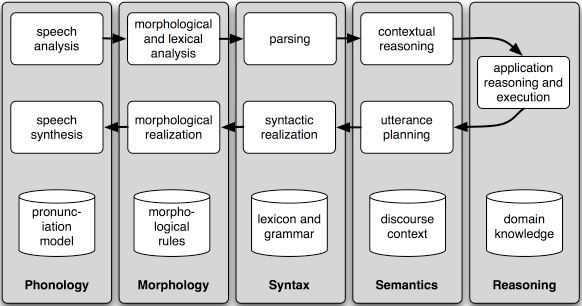
\includegraphics[width=1\textwidth]{pipline}
    \caption{Simple Pipeline Architecture for a Spoken Dialogue System\cite{NLPbook}}
    \label{fig:1}
\end{figure}

In Figure~\ref{fig:1}, \emph{Spoken input (top left) is analyzed, words are recognized, sentences are parsed and interpreted in context, application-specific actions take place (top right); a response is planned, realized as a syntactic structure, then to suitably inflected words, and finally to spoken output; different types of linguistic knowledge inform each stage of the process.}

Dialogue systems give us an opportunity to mention the commonly assumed pipeline for NLP. Figure~\ref{fig:1} shows the architecture of a simple dialogue system. Along the top of the diagram, moving from left to right, is a "pipeline" of some language understanding components. These map from speech input via syntactic parsing to some kind of meaning representation. Along the middle, moving from right to left, is the reverse pipeline of components for converting concepts to speech. These components make up the dynamic aspects of the system. At the bottom of the diagram are some representative bodies of static information: the repositories of language-related data that the processing components draw on to do their work.

\subsection{Textual Entailment}
The challenge of language understanding has been brought into focus in recent years by a public "shared task" called Recognizing Textual Entailment (RTE). The basic scenario is simple. Suppose we want to find evidence to support the hypothesis: \emph{Sandra Goudie was defeated by Max Purnell}, and that we have another short text that seems to be relevant, for example, \emph{Sandra Goudie was first elected to Parliament in the 2002 elections, narrowly winning the seat of Coromandel by defeating Labour candidate Max Purnell and pushing incumbent Green MP Jeanette Fitzsimons into third place}. Does the text provide enough evidence for us to accept the hypothesis? In this particular case, the answer will be "No." We can draw this conclusion easily, but it is very hard to come up with automated methods for making the right decision.
Consequently, some linguistic analysis is crucial. In the previous example, it is important for the system to note that \emph{Sandra Goudie} names the person being defeated in the hypothesis, not the person doing the defeating in the text. As another illustration of the difficulty of the task, consider the following text-hypothesis pair:
\begin{enumerate}[a.]
    \item Text: David Golinkin is the editor or author of eighteen books, and over 150 responsa, articles, sermons and books.
    \item Hypothesis: Golinkin has written eighteen books
    
\end{enumerate}

In order to determine whether the hypothesis is supported by the text, the system needs the following background knowledge: (i) if someone is an author of a book, then he/she has written that book; (ii) if someone is an editor of a book, then he/she has not written (all of) that book; (iii) if someone is editor or author of eighteen books, then one cannot conclude that he/she is author of eighteen books.

\subsection{Information Extraction}
With rise of digital age, there is an explosion of information in the form of news, articles, social media, and so on. Much of this data lies in unstructured form and manually managing and effectively making use of it is tedious, boring and labor intensive. This explosion of information and need for more sophisticated and efficient information handling tools gives rise to Information Extraction(IE) and Information Retrieval(IR) technology. Information Extraction systems takes natural language text as input and produces structured information specified by certain criteria, that is relevant to a particular application. Various sub-tasks of IE such as Named Entity Recognition, Coreference Resolution, Named Entity Linking, Relation Extraction, Knowledge Base reasoning forms the building blocks of various high end Natural Language Processing (NLP) tasks such as Machine Translation, Question-Answering System, Natural Language Understanding, Text Summarization and Digital Assistants like Siri, Cortana and Google Now~\cite{DBLP:journals/corr/abs-1807-02383}.
\begin{figure}[htbp]
    \centering
    \includegraphics[width=.8\textwidth]{ie}
    \caption{Simple Pipeline Architecture for an Information Extraction System~\cite{DBLP:journals/corr/abs-1807-02383}.}
    \label{fig:2}
\end{figure}

Figure~\ref{fig:2} shows the architecture for a simple information extraction system. It begins by processing a document using several of the procedures: first, the raw text of the document is split into sentences using a sentence segmenter, and each sentence is further subdivided into words using a tokenizer. Next, each sentence is tagged with part-of-speech tags, which will prove very helpful in the next step, named entity detection. In this step, we search for mentions of potentially interesting entities in each sentence. Finally, we use relation detection to search for likely relations between different entities in the text.
\subsection{Task Definition}
In our project, we are developing an agent that will follow Bengali instructions to navigate in real-life visual environment.
\begin{itemize}
	\item Inputs: Text based instructions in Bengali language.
	\item Outputs: Mapping instructions and visual observations to actions and execute them in the environment.
\end{itemize}

\section{Motivation}
Computers are great at working with structured data like spreadsheets and database tables. But us humans usually communicate in words, not in tables. That’s unfortunate for computers. A lot of information in the world is unstructured raw text in English or another human language. How can we get a computer to understand unstructured text and extract data from it?

Advances in robotics are enabling progressively more sophisticated, capable technologies to reach large consumer populations. Such systems offer unprecedented potential for AI to help in a variety of human-centric applications such as elder care and household maintenance. However, natural, easy-touse interfaces to such systems, such as those employing natural language, are lagging behind. As robots become more prevalent—and as the need for the services they can offer grows—the importance of allowing non-expert users to interact with them naturally and comfortably increases. Natural language is an excellent modality for end users to give instructions and teach robots about their environments~\cite{ijcai2018-810}. 

As long as computers have been around, programmers have been trying to write programs that understand languages like English. The reason is pretty obvious humans have been writing things down for thousands of years and it would be really helpful if a computer could read and understand all that data. 
NLP is important for scientific, economic, social, and cultural reasons. NLP is experiencing rapid growth as its theories and methods are deployed in a variety of new language technologies. For this reason it is important for a wide range of people to have a working knowledge of NLP. Within industry, this includes people in human-computer interaction, business information analysis, and web software development. Within academia, it includes people in areas from humanities computing and corpus linguistics through to computer science and artificial intelligence~\cite{NLPbook}.

\section{Objectives}
By developing the project, we will learn:
\begin{itemize}
    \item To manipulate large corpora, explore linguistic models and analyze language data.
    \item To use the key concepts from NLP and linguistics to describe and analyse language.
    \item To use data structures and linguistics algorithms in robust language processing software.
    \item To extract knowledge from natural language.
    \item To map instructions from natural language to actions.
    \item To deploy an intelligent agent to execute actions in a particular visual environment.
\end{itemize}





